\chapter{Background}
\label{sec:chapterlabel2}

\section{Recommender Systems}

In recent years, there has been growing focus on the study of Recommender Systems (RSs), where different techniques have been published in order to to address the problem of information overload on the Internet. Consequently, the evolution of RS and the web usually go hand-in hand. Resnick and Varian\cite{resnick1997recommender}  defined RS as systems that help users limit their search by supplying a list of items that might interest them. Such systems has found an active application area for diverse Information Retrieval, Web Mining and Machine Learning techniques that help to solve typical recommendation problems. Additionally,  different RS mechanisms have been categorized depending on the way they analyze the data sources to find affinities between users and items. 

The most general setting in which recommender systems are studied is presented in Figure \ref{fig:iomatrix}. Having a rating matrix of n users and m items representing the current user preferences, the task of a RS is to predict all missing ratings $r_{a,i}$ for the active user a, and then recommend the item(s) with the highest rate\cite{melville2011recommender}. However the user ratings matrix is typically sparse, as most users do not rate most items. Different approaches to solve this task can be categorized into the following types.

\begin{figure}[h]
\centering
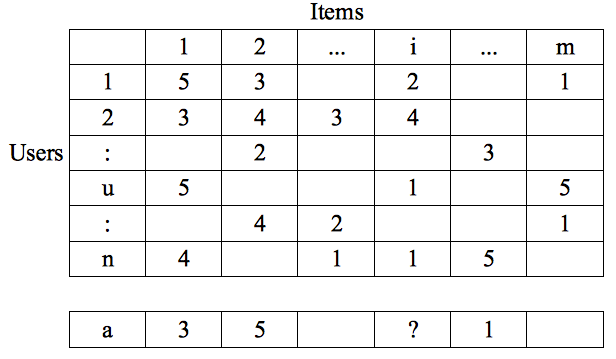
\includegraphics[scale=0.9]{images/uimatrix}
\caption[Typical user rating matrix]{Typical user ratings matrix, where each cell $r_{u,i}$ corresponds to the rating of user u for item i.}
\label{fig:iomatrix}
\end{figure}

\subsection{Collaborative Filtering} 

In Collaborative Filtering (CF) systems, items are recommended by exploiting the similarities amongst several users based on the feedback of previously consumed items. Usually, databases that fit into a CF approach, store the past users interactions in the form of explicit ratings (e.g., 1 to 5 range), or implicit ratings (e.g. a song played by a user, or an item bought by her). In general, CF methods are subdivided into: memory-based and model-based approaches.

\begin{itemize}
\item \textbf{Memory-based CF:} items are recommended using a weighted combination of ratings in a subset of users that are chosen based on their rating similarity to the target user. The most commonly used measure is the Pearson correlation coefficient\cite{resnick1994grouplens}.
%that measures the extent to which there is a linear dependence between the ratings of two users.
Alternatively, the similarity between the ratings of two users (represented as a vector in an m-dimensional space) can be and computed using the Cosine similarity or the adjusted Cosine similarity measure which overcomes the issue of users with different rating behavior schemes\cite{yildirim2008random}. Previous studies found that correlation\cite{breese1998empirical} and adjusted cosine similarity\cite{yildirim2008random} performs slightly better.

Memory-based CF methods have been extended and improved over the years. Linden, Smith, and York\cite{linden2003amazon} proposed an \textit{Item-based} (or item-item) CF method to overcome the problem of dimensionality found when conventional memory-based algorithms cannot scale well when finding similarities between millions of users and items. This approach, which matches a user's rated items using Pearson correlation, lead to faster online systems and improved recommendations.

\item \textbf{Model-based CF:} provides recommendations by using statistical models for predicting user ratings. The most widely used models are Bayesian classifiers, neural networks, fuzzy systems, genetic algorithms, latent features and matrix factorization\cite{bobadilla2013recommender}. For instance, CF methods can be turned into a classification problem, where a classifier is built for each active user representing items as features over users and available ratings as labels. However, latent factor and matrix factorization models have emerged as a state-of-the-art methodology in this class of techniques\cite{koren2009matrix}.

\end{itemize}

%\subsubsection*{Matrix Factorization}
%\label{sec:matrixFactorization}
%
%To reduce the high levels of sparsity in RS databases, matrix factorization in conjunction with dimensionality reduction techniques have been used. Having a sets U of users, and a set D of items, let $\mathbf{R}$ of size $|U| \times |D|$ be the matrix that contains all the ratings that the users have assigned to the items. Assuming that we would like to discover K latent features, the task is to find two matrices $\mathbf{P}$ (a $|U| \times K$ matrix) and $\mathbf{Q}$ (a $|D| \times K$ matrix) such that their product approximates $\mathbf{R}$:
%
%\begin{equation}
%\label{}
%\mathbf{R} \approx \mathbf{P} \times \mathbf{Q^{T}} = \hat{\mathbf{R}}
%\end{equation}
%
%Each row of $\mathbf{P}$ would represent the strength of the associations between a user and the features. Similarly, each row of $\mathbf{Q}$ would represent the strength of the associations between an item and the features. One way to obtain $\mathbf{P}$ and $\mathbf{Q}$ is to first initialize both matrices with some values, and calculate how different their product is to $\mathbf{M}$ by using gradient descent with a regularization term in order to minimize the difference between $\mathbf{R}$ and the predicted preference matrix $\mathbf{\hat{R}}$ (e.g using the Mean Square Error). The update rules and the cost function are defined as follows:
%
%\begin{equation}
%\label{}
%p^{'}_{ik}=p_{ik}+\alpha\frac{\partial}{\partial p_{ik}}e^{2}_{ij}=p_{ik}+\alpha(2e_{ij}q_{kj}-\beta p_{ik})
%\end{equation}
%
%\begin{equation}
%\label{}
%q^{'}_{kj}=q_{kj}+\alpha\frac{\partial}{\partial q_{kj}}e^{2}_{ij}=q_{kj}+\alpha(2e_{ij}p_{ik}-\beta p_{kj})
%\end{equation}
%
%\begin{equation}
%\label{}
%e^2_{ij}=(r_{ij}-\hat{r{ij}})^2=(r_{ij}-\sum_{k=1}^{K}p^{'}_{ik}q^{'}_{kj})^2
%\end{equation}
%
%Another model-based technique combines Latent Semantic Index (LSI) and the reduction method Singular Value Decomposition (SVD) are typically to solve the same problem[***](Using singular value decomposition approximation for collaborative filtering). Although SVD methods provide good prediction results, it is computationally very expensive, therefore it might be only efficient in static off-line settings.

\subsection{Content-based RS}

Content-based (CB) RS (compared to pure CF that only utilizes the user rating matrix) tries to make a better personalized recommendation by exploiting the knowledge about a user (e.g. demographic information), or the properties of items (e.g. genre of a movie). Several approaches have treated this problem as an information retrieval (IR) task, where the content associated with the user's preferences is treated as a query, and the unrated items are scored with relevance/similarity to this query\cite{balabanovic1997fab}. Alternatively, CB-RS has also been treated as a classification task using algorithms such as k-Nearest Neighbors (k-NN), decision trees, and neural networks\cite{pazzani1997learning}

\subsection{Hybrid approaches}

In order to leverage the strengths of both CB-RS and CF methods, several hybrid approaches have been proposed. For instance, Melville et al. presented in \cite{melville2002content} a general framework for content-boosted collaborative filtering, where content-based predictions are applied to convert a sparse user ratings matrix into a full ratings matrix, and then a CF method is used to provide recommendations. In essence, this approach has been shown to perform better than pure CF, pure CB-RS, and a linear combination of the two.

\subsection{The cold-start problem}

The cold-start problem is a common issue that happens in recommender systems when it is not possible to make reliable recommendations due to an initial lack of ratings. There are three kinds of known cold-start problems: new community, new item and new user\cite{bobadilla2013recommender}. However, the latter represents one of the greatest difficulties faced by an RS in operation. Since new users have not yet provided any rating in the RS, they cannot receive any personalized recommendations when using memory-based CF. Usually, when the users enter their firsts ratings they expect the RS to offer them personalized recommendations, but there are not enough ratings yet to be able to make reliable predictions. As a consequence, new users feel that the RS does not offer the service they expected.

This problem is often faced using hybrid approaches such as CF-CB RS, CF-demographic based RS, or CF-social based RS\cite{bobadilla2013recommender}. However, these methods can be combined with clustering techniques over items in order to improve the prediction quality.

\subsection{Trends in Recommendation Systems}

Latest studies in CF showed that combining conceptual (explicit) and usage (implicit) information can improve the quality of web recommendations. Bobadilla et al.\cite{bobadilla2013recommender} presented a taxonomy for RS which unifies the current recommender methods and algorithms that can be applied to incorporate memory-based, social and content-based information into their CF system depending on the type of information available. The taxonomy depicted in Figure \ref{fig:taxonomy}, also detail at its higher levels the current evaluation methods for RS in terms of quality measures, diversity and novelty.

\begin{figure}[h]
\centering
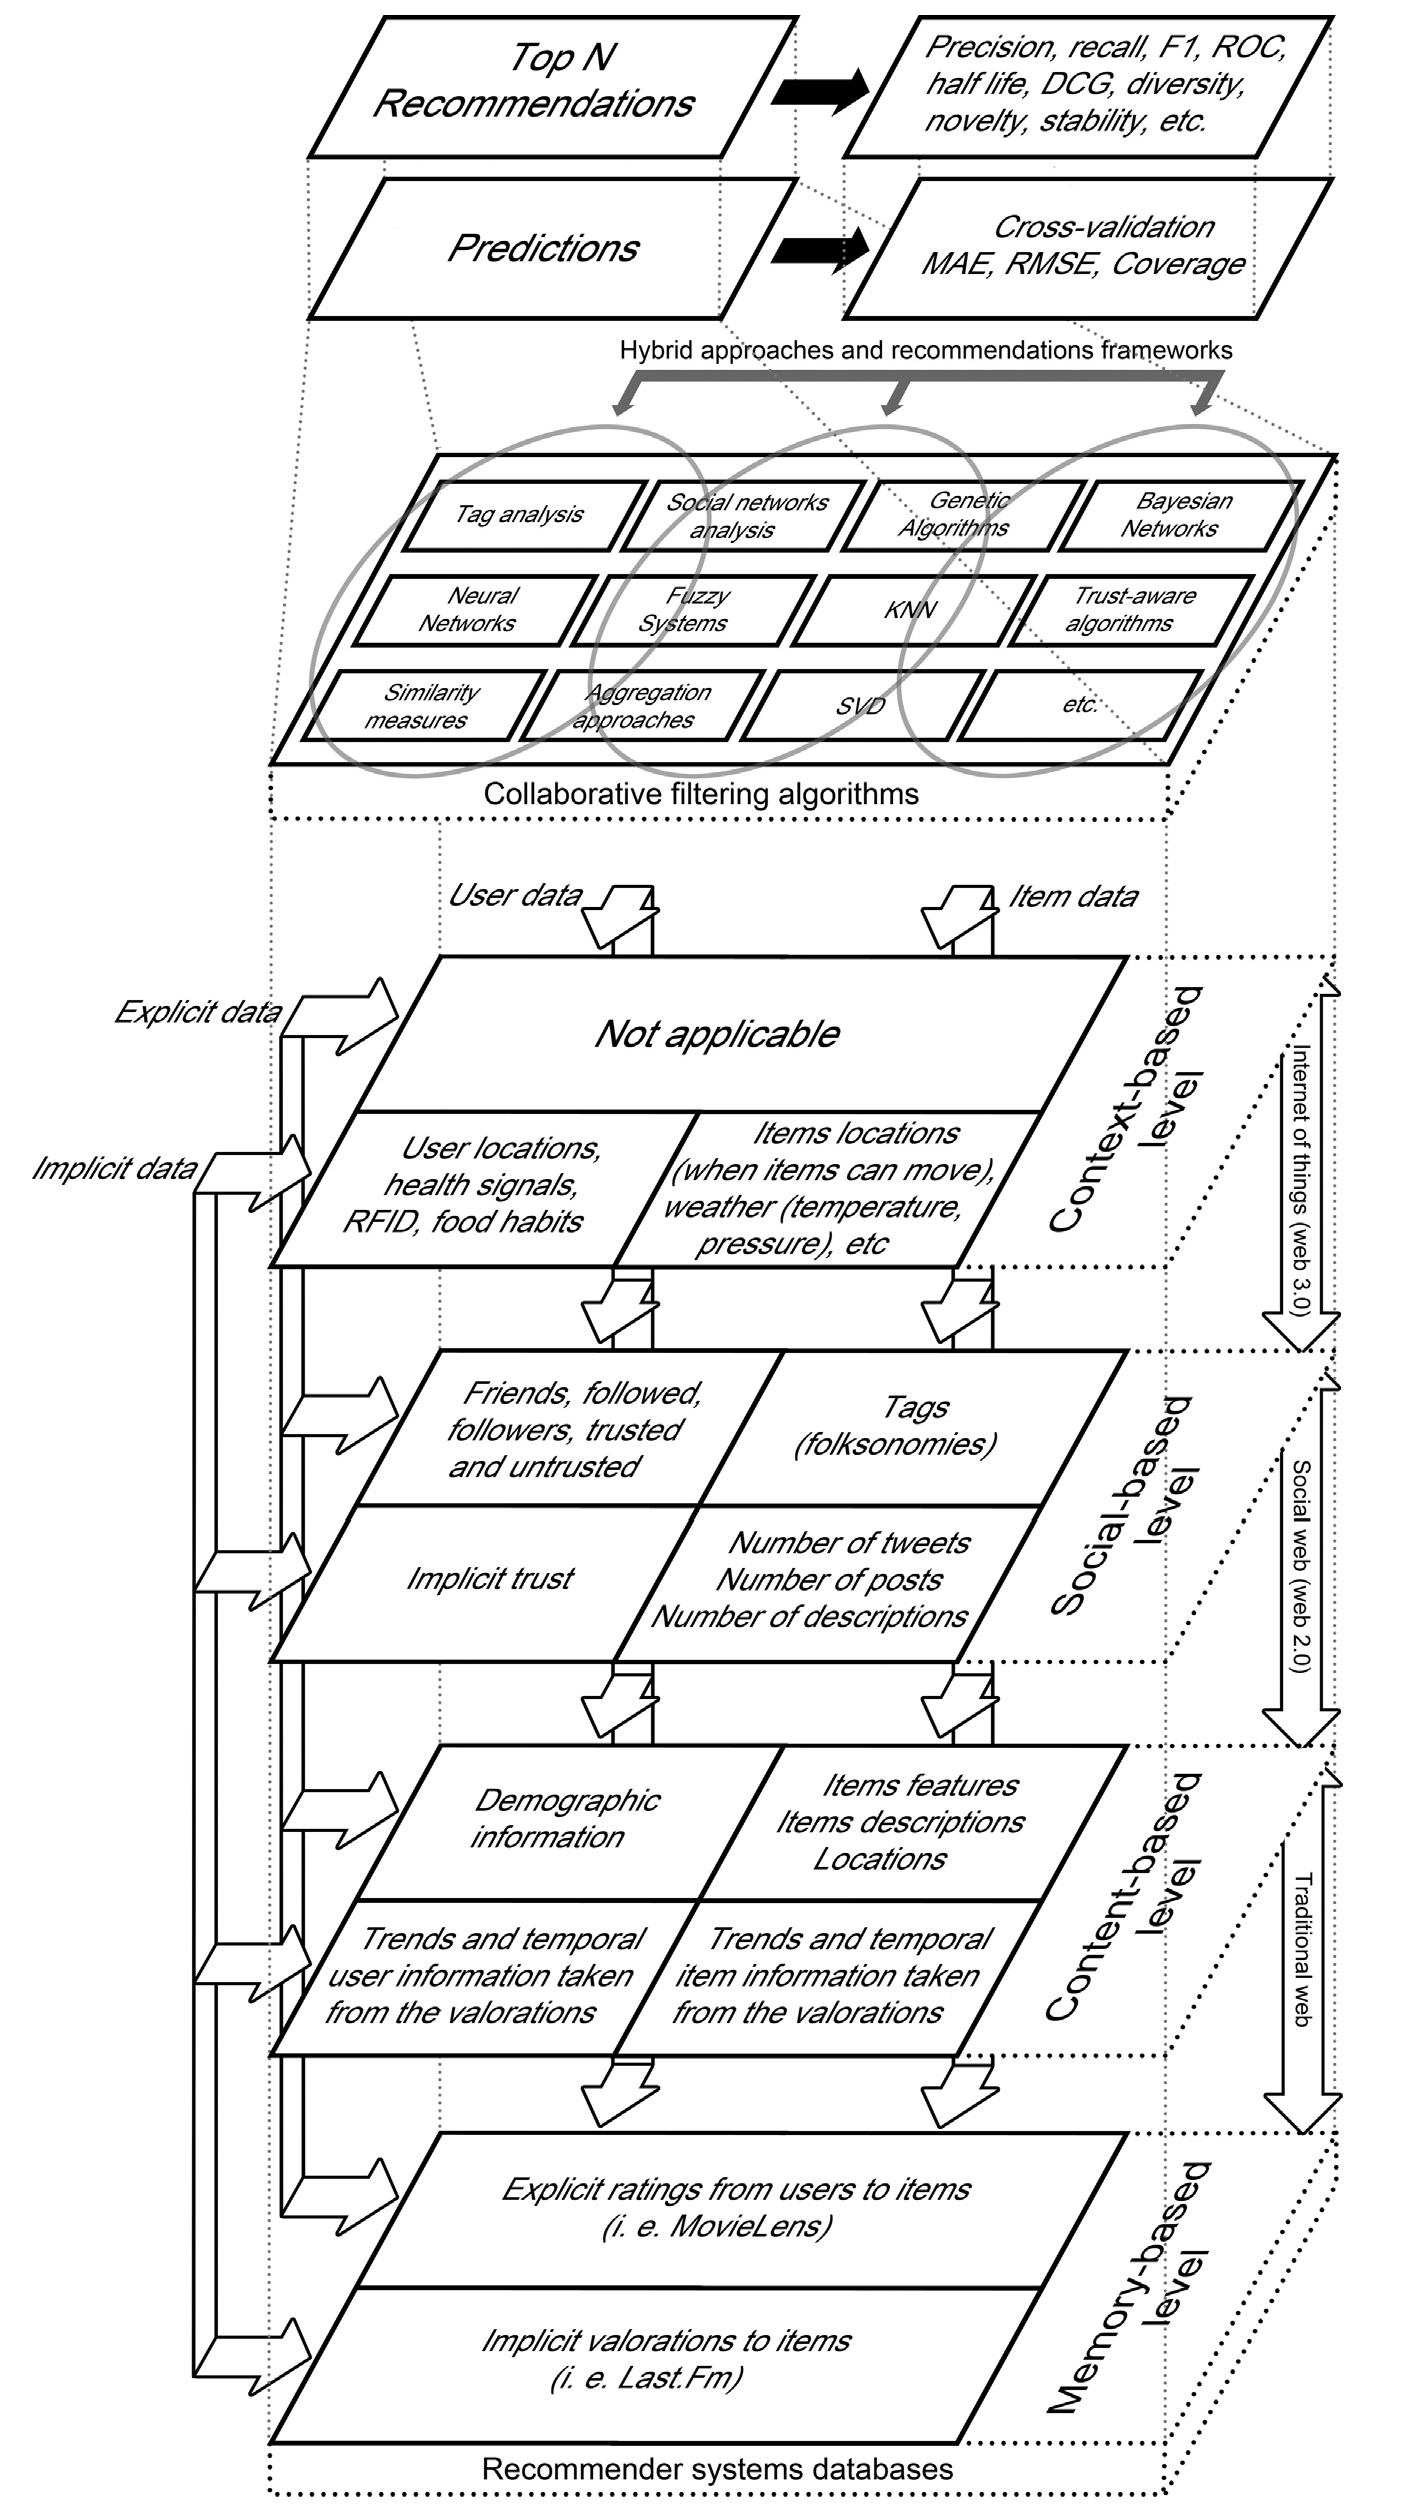
\includegraphics[scale=0.8]{images/taxonomyrs}
\caption[Recommender Systems taxonomy]{Recommender System taxonomy. Source: Recommender systems survey\cite{bobadilla2013recommender}}
\label{fig:taxonomy}
\end{figure}

Moreover, Bobadilla et al. argue that one the most widely used algorithm for CF is the k-nearest neighbors (kNN) model. In general, kNN generates recommendations by executing the following tasks: (1) determine k users neighbors; (2) implement an aggregation approach with the ratings for the neighborhood in items not rated by a; and (3) select the top N recommendations from predictions obtained in step 2.

On the other hand, a more robust model that combines the advantages of Support Vector Machines with factorization models was introduced by Rendle S. in \cite{rendle2010factorization}. The Factorization Machine (FM) model is able to compute all interactions between variables using factorized parameters even in scenarios with huge sparsity like recommender systems. Later, Rendel S. presented in \cite{rendle2012factorization} the \textit{LibFM} software package that implements three learning methods have been proposed for FMs: Stochastic Gradient Descent (SGD)\cite{rendle2010factorization}, Alternating Least-Squares (ALS)\cite{rendle2011fast} and the Markov Chain Monte Carlo (MCMC)\cite{freudenthaler2011bayesian}.

Most recent research like \cite{wang2015collaborative}, made a generalization of recent advances in Deep Learning \cite{bengio2013representation} of the Identically and Independently Distributed (i.i.d.) input and applied it to the non-i.i.d. (e.g. CF-based) input by presenting hierarchical Bayesian models that jointly performs deep representation learning for the content information and CF for the ratings matrix. Additionally, Wu Y. et al. in \cite{wu2016collaborative} proposed a Collaborative Deep Auto Encoders (CDAE) model which formulates the top-N recommendation problem using Denoising Auto-Encoders to learn the latent factors from corrupted inputs. Experiments carried out over different domains have shown that the two deep learning approaches can significantly outperform the state of the art. Therefore, recent research has started to focused on defining deep representational approaches that can lead to better recommendations.

\section{Reinforcement Learning}
Reinforcement learning (RL) \cite{kaelbling1996reinforcement} is a family of machine learning algorithms that optimize sequential decision making processes based on scalar evaluations or rewards. Similarly to an n-armed bandit model\cite{katehakis1987multi}, RL considers the problem as a goal-directed agent interacting with an uncertain environment, where the main objective is to perform actions that maximize the expected sum of future reward for each state in the long term. The most important feature distinguishing RL from other types of learning is that it uses training information that evaluates the actions taken rather than instructs by giving correct actions (like supervised learning algorithms). In other words, an agent must be able to learn from its own experience, like a trial-and-error search.

RL uses a formal framework which defines the continuous interaction in terms of states, actions, and rewards, between the \textit{agent} and an \textit{environment}\cite{sutton1998reinforcement}. At each time step $t$, the agent receives some state representation of the environment $s_t \in \mathcal{S}$, where $\mathcal{S}$ is the set of possible states. Then it selects an action $a_t \in \mathcal{A}(s_t)$ , where $\mathcal{A}(s_t)$ is the set of actions available in the observed state. One time step later, the agent receives a numerical reward $r_{t+1} \in \mathcal{R}$, and the environment turns into a new state $s_{t+1}$. Figure \ref{ig:rlenvironment} shows the whole interaction in an agent-environment interface.

 \begin{figure}[h]
\centering
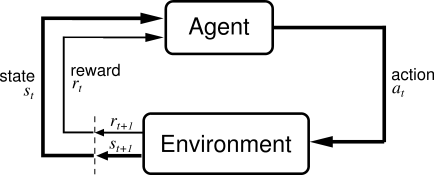
\includegraphics[scale=2]{images/rlenvironment}
\caption[Agent-Environment interface in a Reinforcement Learning problem]{The Agent-Environment interface in a Reinforcement Learning problem. Source: Reinforcement Learning: a Survey\cite{sutton1998reinforcement} }
\label{fig:rlenvironment}
\end{figure}

This framework is intended to be a simple way of representing four essential features of the artificial intelligence problem: (1) a \textit{policy} (commonly stochastic) defines a mapping from the perceived states of the environment to actions to be taken when in those states; (2) a \textit{reward} function maps each state-action pair to a single number that represents how good or bad the new state is for the environment; (3) a \textit{value} function specifies the total amount of reward an agent can expect to accumulate over the future and starting from a given state. This function is considered the most important as it is used by the agent during decision-making and planning; and optionally (4) a model that mimics the behavior of the environment (transitions and rewards) and provides a way of deciding which action to perform considering possible future situations before they are actually experienced.

In general, agents are categorized depending on how the reinforcement learning problem needs to be modeled. \textit{Value-based} and \textit{Policy-based} agents are solely based on the value and policy functions respectively. \textit{Actor-critic} agents use both policy and value functions; \textit{Model-free} agents use policy and/or value function but no model; and \textit{Model-based} agents have all properties mentioned above.

On the other hand, The \textit{return} $R_t$ is defined as the sum of the discounted future rewards over an episode of $T$ time steps that an agent actually seeks to maximize:
\begin{equation}
\label{eq:return}
R_t = r_{t+1} + \gamma r_{t+2} + \gamma^2 r_{t+3} + ... = \sum^{\infty}_{k=0} \gamma^k r_{t+k+1}
\end{equation}
where $\gamma, 0 \leq \gamma \leq 1$ is a discount factor that determines the present value of future rewards

\subsection{Markov Decision Processes}

A Markov Decision Process (MDP) is a model for sequential stochastic decision problems. As such, it is widely used in applications where an autonomous agent is influencing its surrounding environment through actions\cite{shani2005mdp}. It is defined by a tuple $\langle S, A, R, Pr \rangle$ representing a Markov Chain with values and decisions that follows the Markov property: \textit{a state S is Markov if and only if $\mathbb{P}[S_{t+1}|S_t] = \mathbb{P}[S_{t+1}|S_1,...S_t]$. In other words, in a MDP the future is independent of the past given the present}. Therefore, if a reinforcement learning task satisfies the Markov property and the state and action spaces are finite, then it can be modeled as a finite Markov Decision Process.

A particular finite MDP is defined by its state and action sets, a reward function $R$ (equation \ref{eq:expectedRew}) that assigns a real value to each state/action pair, and a state-transition function $Pr$ (equation \ref{eq:transitionsProb}) which provides the probability of transitioning between every pair of states given each action. Altogether, these quantities completely specify the most important aspects of the dynamics of a finite MDP.

\begin{equation}
\label{eq:expectedRew}
\mathcal{R}^a_{ss'} = \mathbb{E} {r_{t+1} | s_t=s, a_t=a, s_{t+1}=s'}
\end{equation}
\begin{equation}
\label{eq:transitionsProb}
\mathcal{P}^a_{ss'} = Pr {s_{t+1} = s' | s_t=s, a_t=a}
\end{equation}

Therefore, the decision-maker's goal is to find an optimal policy $\pi$, such that at each stage of the decision process, the agent needs only to obtain the current state $s$ and execute the action $a=\pi(s)$. Various exact and approximate algorithms have been proposed for estimating the optimal policy $\pi*$, such as policy iteration, value iteration, Monte-Carlo learning, temporal difference, Q-learning, SARSA, etc\cite{kaelbling1996reinforcement}\cite{sutton1998reinforcement}.

\subsection{A model-free Reinforcement Learning Setup}
\label{sec:model-free}

A reinforcement learning setup consists of an agent interacting with an environment $E$ at discrete time steps. At each time step $t$, the agent receives an observation $s_t$, takes an action $a_t$ and receives a reward $r_t$. Additionally, the environment $E$ may be stochastic so it can be modeled as an MDP with a state space $\mathcal{S}$, action space $\mathcal{A}$, an initial state distribution $\rho(s_1)$, transition dynamics $\rho(s_{t+1}|s_t, a_t)$, and reward function $r(s_t, a_t)$. On the other hand, the agent's behavior is defined by a policy $\pi$, which maps states to a probability distribution over the actions $\pi : \mathcal{S} \rightarrow P(\mathcal{A})$. Finally, the return from a state is defined as the sum of the discounted future reward $R_t = \sum^T_{i=t} \gamma^{(i?t)}r(s_i, a_i)$. As the return depends on the actions chosen and therefore on $\pi$, it may be stochastic. 

The goal in reinforcement learning is to learn a policy which maximizes the expected return from a start distribution $J = \mathbb{E}_{r_i,s_i \sim E,a_i \sim \pi}[R_1]$. The action-value function is used in many RL algorithms and describes the expected return after taking an action $a_t$ in state $s_t$ and thereafter following policy $\pi$:
\begin{equation}
\label{eq:action-valueFcn}
Q^{\pi}(s_t, a_t) = \mathbb{E}_{r_{i \geq t}, s_{i > t} \sim E, a_{i > t} \sim \pi} [R_t| s_t, a_t]
\end{equation}

Many approaches in RL opt to represent the action-value function as a recursive relationship using the Bellman equation (eq. \ref{eq:bellmanEq}). Nevertheless, If the target policy is deterministic we can describe it as a function $\mu: \mathcal{S} \leftarrow \mathcal{A}$ and avoid the inner expectation as shown in equation \ref{eq_Qdeterministic}. As the expectation depends only on the environment, it is possible to learn $Q^{\mu}$ off-policy, using transitions which are generated from a different stochastic behavior policy $\mu$.
\begin{equation}
\label{eq:bellmanEq}
Q^{\pi}(s_t, a_t) = \mathbb{E}_{r_{t}, s_{t+1} \sim E} [r(s_t, a_t) + \gamma \mathbb{E}_{a_{t+1} \sim \pi} [Q^{\pi}(s_{t+1}, a_{t+1})] ]
\end{equation}
\begin{equation}
\label{eq_Qdeterministic}
Q^{\mu}(s_t, a_t) = \mathbb{E}_{r_{t}, s_{t+1} \sim E} [r(s_t, a_t) + \gamma Q^{\mu}(s_{t+1}, \mu_{t+1}) ]
\end{equation}

Q-learning\cite{watkins1992q}, is a commonly used off-policy algorithm which uses a \textit{greedy} policy $\mu(s) = argmax_aQ(s, a)$ in order to estimate the action that gives the maximum reward. As the algorithm considers function approximators parameterized by $\theta^Q$, it can be used as an optimizer that minimize the loss:
\begin{equation}
\label{}
L(\theta^Q) = \mathbb{E}_{s_{t} \sim \rho^{\beta}, a_t \sim \beta, r_t \sim E} [(Q(s_t, a_t | \theta_Q) - y_t)^2]
\end{equation}
where $y_t = \mathbb{E}_{s'\sim \mathcal{E}} [r(s_t, a_t) + \gamma max_{a'} Q(s_{t+1}, \mu(s_{t+1}) | \theta^Q)]$. %While $y_t$ is dependent on $\theta^Q$, this is typically ignored.

\subsection{Exploration/Exploitation Dilemma}

One of the challenges that arise in reinforcement learning is the trade-off between exploration and exploitation\cite{kaelbling1996reinforcement}\cite{sutton1998reinforcement}. To obtain a lot of reward, a reinforcement learning agent must prefer actions that has already tried in the past and found to be effective in terms of reward. In order to discover such patterns, it needs to try actions that it has not been selected before. so the agent has to be able to exploit actions that are already known as effective, but it also needs to explore in order to make better action selections in the future.

Na\"{i}ve approaches use a greedy policy $\pi(s) = argmax_aQ(s, a)$ to get the action with maximum reward as a pure exploitative model. However, an $\epsilon$-greedy policy can be considered instead to allow exploration in the environment and improve the estimation of the non-greedy action values. Therefore, the agent will select a random action with a probability $\epsilon$, and will act greedily with probability $1 - \epsilon$ . The advantage of $\epsilon$-greedy policy over greedy policy is that the former continuously explore and improve the chances of recognizing possible actions that can lead to better rewards. 

Nevertheless, this has still been an issue to solve in some reinforcement learning tasks, so research has continuously focused on trying different techniques to solve the exploration/exploitation trade-off that can lead to the discovery of better policies\cite{kaelbling1996reinforcement}.

\section{Recommender Systems and Reinforcement Learning}

Although reinforcement learning seems to have great potential for improving the recommendation problem, it has received relatively little attention and found only limited application. The first experiments on using reinforcement learning techniques were focused on developing recommendation systems for web content using implicit data from server files which stored the navigational logs of the users throughout their contents. 

Ten Hagen et al. \cite{ten2003exploration} considered RL approach with an exploration/exploitation trade-off for discovering unknown areas and automatically improve their recommendation policy to helping users navigate through an adaptive web site. They stated that a model-free algorithm like Q-Learning can become infeasible if the number of actions are relatively high and showed that a greedy policy can indeed lead to a suboptimal recommendation model as the use of such kind of policy function, where the \"best\" actions (e.g with higher probability) are taken, does not always improve the policy. They finally demonstrated that this problem is solved by starting the algorithm with a lot of exploration and gradually reduce the parameter $\epsilon$ as the policy is getting closer to an optimum. Results concluded that a recommender system without exploration potentially can get trapped into a local maxima.

Rojanavasu et al. in \cite{rojanavasu2005new} presented a general framework for web recommendation that learns directly from customer's past behavior by applying an RL process based on the SARSA method and a $\epsilon$-greedy policy. The system was composed of two models: a global model to keep track of customers trends as a whole, and a local model to record the user's individual browsing history. In general, the model treated pages as states of the system and links within a page as actions. To predict the next state, it used a ranking system that is also separated into 2 parts. i) a global ranking system using the data from a $Q_{global}$-matrix obtained from the action-value function and an $\epsilon$-greedy policy that gave the chance for rank new items that have few clicks but may match a user's interest; and ii) a local ranking $Q_{local}$ using an inverse $\epsilon$-greedy policy. The system then finds the final total reward using $Q_{total}=Q_{local} + wQ_{global}$ where $w \in (0-1]$ is a weight hyper parameter of the model. 

Overall, the system provided customers the chance to explore other products than the ones they already visited. Experimental results showed that a value of $\epsilon=0.2$ preserves the balance between exploration and exploitation, meanwhile If $\epsilon < 0.2$ the system will gave small chances to users to explore new items, or otherwise may include products that do not match to the customer's interest ($\epsilon > 0.2$). On the other hand, results also prove that even if the purpose of $Q_{local}$ was to discover new products, it appeared to be less effective than $Q_{global}$.

Shani et al. in \cite{shani2005mdp} argued that it is more appropriate to formulate the problem of generating recommendations as a sequential optimization problem so they described a novel approach for a commercial web site based on MDPs together with a predictive model. The MDP-based recommender system took into account the expected utility and the long-time effect of a particular recommendation. Then it suggested items whose immediate reward is lower, but leads to more \textit{profitable} rewards in the future. However, the benefits of this model are offset by the fact that the model parameters are unknown, randomly initialized and that they take considerable time to converge. So, they defined a strong initial model-based for collaborative filtering, which solves quickly, and that does not consume too much memory.

Before implementing the recommender, they initialize a predictive model of user behavior using data extracted from the web site, and then used it to provide the initial parameters for the MDP. They proposed to use maximum-likelihood estimation with three major enhancements: skipping, clustering, mixture modeling, so the predictive model can be thought of as a first-order Markov chain (MC) of user dynamics in which states correspond to sequences of \textit{k} events (in this case: previous selections) representing relevant information about the users interaction. Then, the transition function described the probability that a user ,whose \textit{k} recent selections were $x_1, . . . ,x_k$ will select the item $x'$ next.

Authors experimented with small values of \textit{k} ($k \in [1-5]$) in order to overcome data sparsity and MDP solution complexity issues. Moreover, enhancements on the maximum-likelihood n-gram formulation showed to be useful to find a good estimate of the transition function for the initial predictive model without suffering the problem of data sparsity and bad performance presented on other model variations.

%The proposed maximum-likelihood estimation include three major enhancements. First, a form of skipping based on the observation that the occurrence of the sequence $x_1,x_2,_x3$ lends some likelihood to the sequence $x_1,x_3$. In other words, after initializing the counts of each state transition using the observed data, for any given user sequence $x_1,x_2, ...,x_n$, they added a fractional count $1/2^{( j-(i+3))}$ to the transition from $s=\langle x_i,x_{i+1},x_{i+2}\rangle$ to $s'=\langle x_{i+1},x_{i+2},x_j\rangle$, for all $i+3 < j ?n$, which acts as a diminishing probability of skipping a large number of transactions in the sequence. Equation \ref{eq:trMCSkipping} shows the updated formulation of the (normalized )maximum-likelihood estimation, where $count(s,s')$ is the fractional count associated with the transition from s to s'.
%
%\begin{equation}
%\label{eq:trMCSkipping}
%tr_{MC}^{base}(s,s')=\frac{count(s, s')}{\sum_{s'}count(s, s')}
%\end{equation}
%
%The second enhancement exploits the similarity  of sequences in a form of clustering. The idea is that the likelihood of transition from $s$ to $s'$ can be predicted by occurrences from $t$ to $s'$, where $s$ and $t$ are similar. Equation \ref{eq:simTr} define the similarity of states $s_i$ and $s_j$ where $\delta(\dot, \dot)$ is the Kronecker delta function and $s^m_i$ is the m-th item in state $s_i$. Then, the similarity count from state $s$ to $s'$ was defined using equation \ref{eq:simCountTr}. Finally, the new transition probability from $s$ to $s'$ given by equation \ref{eq:newTr} yielded the best results during evaluation.
%
%\begin{equation}
%\label{eq:simTr}
%sim(s_i, s_j)=\sum_{m=1}^{k}\delta(s_i^m, s_j^m) \cdot (m+1)
%\end{equation}
%\begin{equation}
%\label{eq:simCountTr}
%simcount(s, s')=\sum_{s_i} sim(s, s_i) \cdot tr^{base}_{MC}(s, s')
%\end{equation}
%\begin{equation}
%\label{eq:newTr}
%tr_{MC}(s, s')=\frac{1}{2}tr^{base}_{MC}(s, s') + \frac{1}{2}\frac{simcount(s, s')}{\sum_{s''}simcount(s, s'')}
%\end{equation}
%
%Due to larger values of k lead to states that are more informative whereas smaller values of k lead to states with more statistical meaning, they added as a third enhancement a finite mixture modeling (e.g. combine a trigram, a bigram and a unigram into a single model) in a way to balance these conflicting properties by mixing k models, where the \textit{i-th} model looks at the last i transactions. In addition, they applied mixture weights during experiments as $\pi_1 = · · · = \pi_k = 1/k$ so the generation of the models for smaller values entails little computational overhead.

%An evaluation on the accuracy of the predictive model was performed using real user transactions and browsing paths (from web logs) from the commercial store web site. Besides, they compared different variations of their enhancements on the MC approach with other models like i)both sequential and non-sequential form of the \textit{Microsoft Commerce Server 2000}(Heckerman et al. (2000))[***] (local distributions are probabilistic decision trees); and ii)unordered versions of MC models. Results outlined that the MC models using skipping, clustering, and mixture modeling yielded better results than any other other variation of model \textit{i}. Sequence-sensitive models outperformed the accuracy of non-sequential models, while MC models were superior to the predictor models. and the skipping enhancement was only beneficial for the transactions data set

On the other hand, 
%the MDP-based recommender system, models the recommendation process as a sequence of states and attempts to optimize it. Here, the predictive model played an important role in the construction of the model as it provides the probability, denoted by $Pr_{pred}(x|x_1, . . . ,x_k)$, that a user purchase a particular item x given her sequence of past purchases  $x_1, . . . ,x_k$. 
the components of the reinforcement learning model were defined as follows: a) the states are the \textit{k}-tuples of items purchased; b) actions correspond to a recommendation of an item; c) rewards depends only on the last item defining the current state, where its net profit was used; and d) the transition function as the stochastic element of the model that estimates the user's actual choice.% In brief, equation \ref{eq:trMDP} represents the transition function or the probability that a user will select item $x''$ given that item $x'$ is recommended in state $\langle x_1,x_2,x_3 \rangle$.

%\begin{equation}
%\label{eq:trMDP}
%tr^1_{MDP}(\langle x_1,x_2,x_3 \rangle,x',\langle x_2,x_3,x'' \rangle) 
%\end{equation}

In order to solve the MDP problem, a policy iteration algorithm was used as the defined state space presented certain characteristics that lead to fast convergence.
%Indeed, tests performed on real data showed that the policy iteration converges after a few iterations.
%: i) the inherent directionality that transitions showed are useful to reduce the running time of the solution algorithm; ii) the computation of an optimal policy is not sensitive to variations in the number of \textit{k} past transactions a state represent; iii) ignoring unobserved states by maintaining transition probabilities only for states where a transition actually occurred; and  iv) using the independence of recommendations or Markov property, where the probability that a user buys a particular item depends only on her current state, allowing the algorithm to handle large action spaces.
The transition function was carefully initialized in order to be fairly accurate when the system was first deployed to avoid the cold-start problem,causing states that are infrequently observed to be updated faster than already observed states. Moreover, when the first transition to a state is observed, its probability is initialized to 0.9. In this way, the system balances the need to explore unobserved items in order to improve its model by recommending non-optimal items occasionally until getting their actual counts.
Finally, to update the model, the system used an off-line approach which keeps track of the recommendations and the user selections and build a new model at fixed time intervals (e.g. once a week).


%So, to re-estimate the transition function at time $t+1$ the following counts are obtained:
%
%\begin{equation}
%\label{eq:countIn}
%c^{t+1}_{in}(s, r, s \cdot r) = c^{t}_{in}(s, r, s \cdot r) + count(s, r, s \cdot r)
%\end{equation}
%\begin{equation}
%\label{eq:countOut}
%c^{t+1}_{out}(s, r, s \cdot r) = c^{t}_{out}(s, r, s \cdot r) + count(s, s \cdot r) - count(s, r, s \cdot r)
%\end{equation}
%\begin{equation}
%\label{eq:countTotal}
%c^{t+1}_{total}(s, s \cdot r) = c^{t}_{total}(s, r, s \cdot r) + count(s, s \cdot r)
%\end{equation}
%\begin{equation}
%\label{eq:modelProb1}
%tr(s, r \in R, s \cdot r) = \frac{c^{t+1}_{in}(s, r, s \cdot r)}{c^{t+1}_{total}(s, s \cdot r)}
%\end{equation}
%\begin{equation}
%\label{eq:modelProb2}
%tr(s, r \notin R, s \cdot r) = \frac{c^{t+1}_{out}(s, r, s \cdot r)}{c^{t+1}_{total}(s, s \cdot r)}
%\end{equation}
%\begin{equation}
%\label{eq:initIn}
%c^{0}_{in}(s, r, s \cdot r) = \xi_S \cdot tr(s, r, s \cdot r)
%\end{equation}
%\begin{equation}
%\label{eq:initOut}
%c^{0}_{out}(s, r, s \cdot r) = \xi_S \cdot tr(s, r, s \cdot r)
%\end{equation}
%\begin{equation}
%\label{eq:initTotal}
%c^{0}_{total}(s, s \cdot r) = \xi_S 
%\end{equation}
%where Equation \ref{eq:countIn} corresponds to the number of times a recommendation r was accepted in state s, equation \ref{eq:countOut} is the number of times a user select item r in state s even though it was not recommended, equation \ref{eq:countTotal} is the number of times a user pick item r while being in state s, regardless of whether it was recommended or not, and finally, equations \ref{eq:modelProb1} and \ref{eq:modelProb2} represent the actual probability that a user will select item r given state s when r was recommended or not respectively. 

%The transition function had to be carefully initialized in order to be fairly accurate when the system was first deployed to avoid the cold-start problem, so the at time $t=0$ were calculated using equations \ref{eq:initIn} \ref{eq:initOut} \ref{eq:initTotal}, where $\xi_s= 10 \cdot count(s)$, causing states that are infrequently observed to be updated faster than already observed states. Moreover, when the first transition to a state $s \cdot r$ is observed, its probability is initialized to 0.9 the probability of the most likely next item in state s with $\xi_s =10$. In this way, the system balances the need to explore unobserved items in order to improve its model by recommending non-optimal items occasionally until getting their actual counts.  

Experiments demonstrated that a deployed system using three mixture components (combined using an equal weight), with history length $k \in [1,3]$ was able to generate 28\% higher average user reward compared to pure MC model, while in terms of computational costs, the MDP-based model was built quickly and provided fastest recommendations at the price of more memory use. All in all, the off-line predictive model approach provided an adequate initial performance that overcomes the cold-start problem, however, authors avoid using some form of reinforcement learning technique as they argued that at that time, its implementation requires many calls and computations by a recommender system online, which lead to slower responses and undesirable results for the web site owner.

A machine learning perspective, introduced by Taghipour et al. in \cite{taghipour2007usage}, used an off-line reinforcement learning model to solve the recommendation problem using the Q-Learning algorithm while employing concepts and techniques commonly applied in the web usage mining domain. They argued that this method is appropriate for the nature of web page recommendation problem as it provides a mechanism which is constantly learning, does not need periodic updates, can be easily adapted to changes in the website structure and new trends in users behavior.

The RL problem formulation was considered as as a competition between different recommender systems to gather more points, 
%than a 2-player game, as in the recommender system environment, self-play, a typical technique used in training RL systems[***], cannot be used to train the system so the system needed of actual web usage data for training. 
together with a stochastic model with the following properties: 

\begin{itemize}
\item \textit{states:} showing the history of pages visited by the user so far. For this case, a notion of N-Grams was adopted and a sliding window of size $w$ was set to limit the page visit sequences to a constant number and avoid large state spaces.
\item \textit{actions:} consisting of a single page recommendation at each state.
\item \textit{policy:} rewards actions positively if it recommends a page that will be visited in one of the consequent states
\item \textit{reward} function: defined as $r(s, a) += reward(Dist(Rs', p), Time(p^v_w))$, where $Dist(Rs', p)$ is the distance of page p from the end of the recommended pages list to state $s'$, and $Time(p^v_w)$ indicates the time user has spent on the last page of the state. Finally, the $reward(Dist, Time)$ function was defined as a linear combination of both values: $reward(Dist,  Time) = \alpha \times dist + \beta \times Time$ with $\alpha + \beta = 1$.
\end{itemize}

%As the model did not have a predetermined reward function $R(s, a)$ or a transition function $\delta(s, a)$ to give the next state, the reward was estimated by considering that each state s is formed by two sequences $V_s =\langle p^V_{s,1}, p^V_{s,2},..., p^V_{s,w} \rangle$, and $R_s =\langle p^R_{s,1}, p^R_{s,2},..., p^R_{s, n} \rangle$, indicating the sequence of visited and previously recommended pages respectively, where $p^V_{s, i}$ , indicates the ith visited page in the state and $p^R_{s, i}$ indicates the ith recommended page in the state s, Additionally, they had two considerations in the implementation of the reward function: i) only the occurrence of the last page visited in the recommended pages list in state $s'$ is used to reward the action performed in the previous sate $s$, and ii) the time the user spends on a page, assuming that the more time a user spends on a page the more interested. So, the reward function was defined as follows:
%\begin{enumerate}
%\item Assume $\delta(s, a) = s'$
%\item $P_R = V_{s', w} \cap R_{s'}$
%\item if $p \neq \emptyset$
%\item For page $p$ in $P_R$
%\begin{enumerate}
%\item $r(s, a) += reward(Dist(Rs', p), Time(p^v_w))$
%\end{enumerate}
%\end{enumerate}
%where $Dist(R_i, p)$ is the distance of page p from the end of the recommended pages list and $Time(p^v_w)$ indicates the time user has spent on the last page of the state. Finally, The $reward(Dist, Time)$ function was defined as a linear combination of both values as $reward(Dist,  Time) = \alpha \times dist + \beta \times Time$ with $\alpha + \beta = 1$.
%
%Subsequently, the  definition of the learning algorithm also took into consideration the following characteristics: 1) the Q-Learning algorithm given by equation \ref{eq:QLearningalg} was proposed as an update rule and the structure to estimate how successful a prediction can be. Here, the decreasing value of $\alpha_n$ caused these values to gradually converge and decreases the impact of changing reward values as the training continues; 2) an $\epsilon$-greedy action selection was picked as it is important to add some exploration of the state space especially at the beginning of the training; 3) the algorithm followed a TD(0) off-policy learning[***] procedure, as the maximum Q value of the next state is considered when estimating the future reward; and 4) the computation of $r(s, a)$ suffered a slightly change by considering value of $Q(s',a)$ with a coefficient $\gamma$ in order to propagate the value of performing a specific action beyond the limits imposed by the $w$. As the authors mentioned in their work: "the basic idea is that when an action/recommendation is appropriate in state Si, indicating the recommended page is likely to occur in the following states, it should also be considered appropriate in state $S_{i-1}$ and the actions in that state that frequently lead to $S_i$". During the training phase, the described algorithm converged after a few thousand (between 3000 and 5000) visits of each episode or user session.
%
%\begin{equation}
%\label{eq:QLearningalg}
%Q_n(s, a )= [(1 - \alpha_n)Q_{n-1}(s, a) + \alpha_n[r(s, a)  + \gamma \max_{a'} Q_{n-1}(\delta(s, a), a')]
%\end{equation}
%with
%\begin{equation}
%%\label{}
%\alpha_n = \frac{1}{1 + visits_n(s, a)}
%\end{equation}
%
%For the purpose of performing a set of experimental evaluations of the proposed model, simulated log files generated by a web traffic simulator were used to train and tune the rewarding functions. The metric used for each evaluation were Recommendation Accuracy, Coverage (similar to precision and recall metrics) and Shortcut Gain (measures how many page-visits users can save if they follow the recommendations). First of all, an experiment with different values of $w$ showed that fixed window size of 3 as recommendation history resulted on better accuracy and shortcut gain, so this value was set for the rest of system evaluations. Next, they experimented the impact of gradually increasing (in steps of 5\%) the coefficient $\alpha$ of parameter \textit{Dist} in the reward function, resulting on both higher accuracy and higher shortcut gain for values up to 15\%. This matched the natural consequence of adding a bounded size of window on recommendations history. Finally, a set of experiments also tested the system performance by increasing the coefficient $\gamma$ in the reward function, obtaining an increase of the accuracy until reaching an upper bound (around 0.20\%) where it began to drop, while the shortcut gain increased steadily up to a point where recommendations became so inaccurate.

The proposed off-line RL method used a simplified formulation of the recommendation problem but it obtained much better results compared with two baselines methods: association rules and item-based collaborative filtering (with probabilistic similarity measure). As the coverage increase, naturally accuracy decrease in all systems, but the RL approach outperformed the other two systems displaying a lower rate in which its accuracy decreased. Authors concluded that the algorithm is a good candidate for solving the recommendation problem as it does not rely on any previous assumptions regarding the probability distribution of visiting a page after having visited a sequence of pages, and that the nature of the problem matches perfectly with the notion of delayed reward (known as temporal difference). Additionally, they suggested that in order to produce better results it could be possible to use a more complicated formulation of the reward function such as a neural networks, rather than a linear combination of factors.

Later in \cite{taghipour2008hybrid} they exploited the previous RL framework and present a hybrid web recommendation method enriched with semantic knowledge about the usage behavior and thus obtain a more generalized solution regarding to the usage data it has. The new system used the incremental Document Conceptual Clustering\cite{godoy2006modeling} algorithm to map pages to higher level concepts, and thus exploit the hierarchical and conceptual document clustering to provide a semantic relationship between them in combination with the usage data in a user session.

Therefore, new states consist of a sequence of concepts visited by the user, while actions are recommendation of pages that belong to a specific concept. This definition resulted in a much smaller state-action space as the size of the state space is now dependent on the number of distinct page clusters. Finally, the new reward function takes into account the content similarity of the recommended and visited pages along with the usage-based reward defined in the previous approach.

%Now, an action $a$ recommending a concept $c$ is rewarded if the user visits a page belonging to concept $c$ later in his browsing session. The new reward function shown in  equation \ref{eq:hybridreward} takes into account the content similarity of the recommended and visited pages, where CBR represents the content-based reward of an action (which is equal to the similarity score between concepts) defined in equation \ref{}, and UBR is the usage-based reward defined in the previous approach.
%
%\begin{equation}
%\label{eq:hybridreward}
%UBR(Dist(R_{s'} , r),Time(P_{t+1})) \times CBR(r, C(P_{t+1}))
%\end{equation}
%\begin{equation}
%\label{}
%l(c) = -log \mathcal{p}(c)
%\end{equation}
%\begin{equation}
%\label{}
%Sim(c_1, c_2) = max_{a \in LCA} {l(a)}
%\end{equation}

The modified algorithm do not make predictions based on weak usage patterns as the new states represented a generalized view of many single visit sequences. Furthermore, evaluation results showed the flexibility of the new RL approach to incorporate different sources of information in order to improve the quality of recommendations.

%\textbf{Improving adaptation of ubiquitous recommender systems by using reinforcement learning and collaborative filtering} proposed a learning system for Context-based Recommender System (CBRS)[***] by modeling an MDP agent which combines a hybrid Q-learning algorithm (HQL), collaborative filtering and case-based reasoning techniques in order to define a \textit{contextual} recommendation process based on different context dimensions (cognitive, social, temporal, geographic). It addressed the following problems that came out in recommender systems: a)avoid the intervention of experts as the use of the Q-learning algorithm does not need initial user?s information; b)reduce the cold start problem thanks to the ability of the Q-learning algorithm to explore the knowledge of other users in the same context by using CF; c)accelerate the learning process by mixing Q-learning with case-based reasoning techniques (reuse of cases yields to faster user satisfaction); and d)an exploration strategy allows recommendations to adapt to the user's interest evolution.
%
%As a result, the model was based in three main algorithms. First, a hybrid-based CF approach which combines the advantages of the memory-based (fill the missing rating values of the user-item matrix) and model-based CF (form the nearest neighbors of each item). Second, the Case based reasoning (CBR)[***] algorithm was picked as it uses knowledge of previous cases to solve new problems, by finding a similar past case and thus reusing it to solve the current situation. Finally, the Q-learning algorithm was improved by: i)reusing past cases information gathered from the CBR, and ii)giving the ability to use information from other users sharing the same interests, by extending the $\epsilon$-greedy strategy to select a random action based on the similarity of user profiles (obtained from the CF algorithm).
%
%The global mechanism of a context-based recommender system (CBRS) which uses the HyQL algorithm was composed mainly by the following modules:
%
%\textbf{sensing module:} detects time, location, cognitive and social dimensions of the context.
%
%\textbf{thinking module:} composed by an abstraction phase that is based on inference rules defined on temporal and space ontologies, and an aggregation phase the two dimensions.
%
%\textbf{reasoning module:} chooses an action based on the HyQL algorithm
%
%Finally, evaluations comparing the Q-learning and HyQL with respect to solving the cold start problem were performed, and consisted on testing the precision of the first 100 trials of the system starting when the user is connected to the system. In General, results showed that the precision of HyQL was greater than the precision of Q-learning, demonstrating that this approach is a good candidate to be used in the recommender system problem. However, as the system implementation depends on the context data, it needs of a hand-crafted feature creation process in order to be used on different situations.

%\textbf{Exploration in Interactive Personalized Music Recommendation: A Reinforcement Learning Approach} formulated an interactive and personalized music recommendation approach as a reinforcement learning task based on the multi-armed bandit problem, where songs were treated as arms and user ratings as payoffs, and the objective function was set to maximize the cumulative reward of a targeted user over the long term. The model considered the exploration-exploitation trade-off and a Bayesian model in order to deal with both audio content and the novelty of recommendations and thus learn the user musical preferences online based on their feedback. 
%
%The model differs from other approaches in three aspects: i)it is based on audio content; ii)the model is highly efficient as it allows easy online updates; and iii)the model is evaluated based on online real-life user interaction data and does not need a test dataset. Moreover, each recommendation serves two objectives: (1) satisfy the user?s current musical taste, and (2) obtain user feedback needed to improve future recommendations. Even though authors mentioned that an MDP formulation can model a broader range of problems than the multi-armed bandit, it requires much more data to train and is often more computationally expensive.
%
%Their choice to work with a the content-based approach rather CF was justified for the following reasons. First, due to the bayesian nature of their formulation, methods for matrix factorization (MF) are much more complicated than the proposed linear model. Second, MF often needs of large amount of data for training. Third, existing Bayesian MF methods are inefficient for online updating, so they do not fit in a bandit model which is updated once a new rating is obtained, Fourth, a content-based method does not suffer of the new song problem. Finally, content-based approaches capture causality within music content rather than pure correlation that CF methods offer.
%
%Subsequently, the interactive, personalized recommender system used a reinforcement learning task called the multi-armed bandit[***] which addressed both the exploration-exploitation trade-off and playlist generation with a single unified model. Whereas some RL models considered only a greedy strategy that does not actively seek fort user feedback, resulting in suboptimal recommendations over the long term, this model takes into account the uncertainty of both the mean and the variance of the rating distribution, allowing the recommender to explore user preferences actively rather than merely exploiting the available rating information. An approach better than the typical $\epsilon$-greedy method to solve of the multi-armed bandit problem, is the use of the Upper Confidence Bound (UCB)[***] algorithm, but it requires an explicit form of the confidence bound that is difficult to derive in the case of music recommendation.
%
%The personalized music rating model was focused on audio content and novelty. The former considers the overall preference of a song and is represented by the linear function $U_c = \mathbf{\theta'x}$ where $\mathbf{x}$ is the feature vector of the audio content and $\mathbf{\theta}$ is the user preference in different music features (it was considered constant over time). On the other hand, the novelty factor was defined after examining the song's repetition distribution of 1000 users? listening histories collected from the Last.fm dataset. Results showed that most of the songs a user listens to are repeats and that the frequency distribution approximately follows the Zipf?s law[***], where only a small set of songs are repeated most of the time. As a consequence, it was assumed that the novelty of a song decays immediately after it is listened to and then gradually recovers according to the function $U_n = 1 - e^{-t/s}$, where s is a recovery speed (unknown) parameter learned from user interactions and $e^{-t/s}$ is the well-established forgetting curve[***] that measures user's memory retention of a song. In other words, novel songs are those of which that at a certain time a user has little or no memory. It is important to emphasize that the definition of this factor could be different or not applicable to other recommendation contexts than the musical environment.
%
%Overall, the rating model, defined in equation \ref{eq:combinedRatingModel}, assumed that a rating is formed as the combination of the user?s preference of the song?s content and the dynamically changing novelty. Hence, each user was represented by a set of parameters $\Omega = \{\theta, s\}$, where $\Omega$ needs to be estimated from historical data, so uncertainty had to be taken into account. 
%
%\begin{equation}
%\label{eq:combinedRatingModel}
%U = U_cU_n = \mathbf{\theta'x}(1 - e^{-t/s})
%\end{equation}
%
%With this in mind, the new problem formulation was solved using the Bayesian Upper Confidence Bound (Bayes-UCB)[***] algorithm. In The Bayes-UCB, the true expected payoff $U_i$ defined in equation \ref{eq:expectedRatingUCB} for arm \textit{i} is treated as a random variable and the posterior distribution $p(U_i|\mathcal{D})$ of $U_i$ given the history of payoffs $\mathcal{D_l} = \{(\mathbf{x_i}, t_i, r_i)\}^{l}_{i=1}$ is predicted using equations\ref{eq:posteriorDistrOmega} and \ref{eq:posteriorDistrU}. Finally, the Bayes-UCB recommends song $k^*$ that maximizes the quantile function $argmax_{k=1...|S|} Q(\alpha, P(U_k|D_l))$ where Q satisfies$\mathcal{P}[Uk \leq Q(\alpha, P(U_k|D_l))] = \alpha$ and $\alpha = 1 - \frac{1}{l+1}$
%
%\begin{equation}
%\label{eq:expectedRatingUCB}
%\mathcal{E}[R_i] = U_i = \mathbf{\theta'x_i}(1 - e^{-t_i/s})
%\end{equation}
%\begin{equation}
%\label{eq:posteriorDistrOmega}
%p(\mathbf{\Omega}|D_l) \propto p(\mathbf{\Omega}) p(\mathbf{\Omega}|D_l)
%\end{equation}
%\begin{equation}
%\label{eq:posteriorDistrU}
%p(U_k|D_l) = \int p(U_k|\mathbf{\Omega}) p(\mathbf{\Omega}|D_l) \mathbf{d\Omega}
%\end{equation}
%
%Since equation \ref{eq:posteriorDistrOmega} does not have a closed-form solution, a Markov Chain Monte Carlo (MCMC)[***] should be used as an approximate inference algorithm. However, authors argued that its performance is very low and users could wait for up to a minute until the MC converges. Hence, they developed a Bayesian model using a piecewise-linear function approximation, as well as a variational inference algorithm to approximate posterior distribution of $\Omega$. For more details about the model definition, please refer to section 4.2 in [***](this paper). Authors mentioned that even if the model just considered audio content and novelty of music on its definition, other factors like diversity, mood or genre could be also approximated by linear functions and then added to it. All in all, the defined approximate Bayesian model was used to obtain the fixed-level quantile of $p(U_i|\mathcal{D})$ and thus estimate the expected payoff and confidence bound of the conceptual Bayes-UCB.
%
%Evaluations of both efficiency and effectiveness were carried out over six recommendation algorithms and models (Random, LinUCB-C (Content-based), LinUCB-CN (Content and novelty based), Bayes-UCB-CN, Bayes-UCB-CN-V (Variational Inference), and Greedy-CN) demonstrating that the proposed approaches were accurate and highly efficient. The effectiveness study used the \textit{regret}[***] metric to compare the algorithms, showing that the Bayes-UCB-based algorithms performed better than Greedy-CN due to the balance of exploration and exploitation it offers, whereas the good performance of the Bayes-UCB- CN-V indicated that the piecewise-linear approximation and variational inference were appropriately defined. Moreover, results in the efficiency study empirically proved that the developed variational inference algorithm was 100 times faster than the MCMC. Additionally, a user study and an overall evaluation of recommendation performance dropped good conclusions. Results showed that the bandit approach with the novelty factor addressed the cold-start problem improving the recommendation performance.
%
%To sum up, this work was considered by the authors as the first to balance exploration and exploitation based on reinforcement learning and the multi-armed bandit, and thus improve recommendation performance by addressing the cold-start problem in music recommendation without relying on additional (contextual information). An approximation to the rating model and the new probabilistic inference algorithms helped to achieve real-time recommendation performance that could be generalized to other recommenders and/or media types. Finally, authors suggested that this work could be extended to model the correlations between different users to further reduce the amount of exploration by using hierarchical Bayesian models. On the other hand, if people prefer to boost the performance of CF, they suggested to exploit the exploration/exploitation trade-off idea by using the latent features learned during the matrix factorization rather than the audio features and keep other parts of the proposed system unchanged.
%
%\textbf{ENHANCING COLLABORATIVE FILTERING MUSIC RECOMMENDATION BY BALANCING EXPLORATION AND EXPLOITATION} extended the work presented above by introducing exploration into the CF context. The approach used a Bayesian graphical model that takes into account the CF latent factors and novelty of recommendation, as well as a Bayesian inference algorithm to efficiently estimate the posterior rating distributions.
%
%Authors argued that their previous work, based on a content-based approach, had experienced the following drawbacks: (i) the personalized user rating model suffer of a semantic meaning between low-level audio features and high-level user preferences; (ii) it is difficult to determine which acoustic features are actually effective in the music recommendation scenario; and (iii) recommendation of songs under this approach lacks of variety due to most of them are acoustically similar. Therefore, they presented a memory-based CF approach using matrix factorization in order to improve recommendations.
%
%Recalling the definition of Matrix factorization in Section \ref{sec:matrixFactorization}, this method characterizes users and songs by vectors of latent factors $\mathbf{u_i}$ and $\mathbf{v_j}$ respectively with $i \in [1, m], j \in [1, n]$. In order to learn the latent feature vectors, the system used equation \ref{eq:matrixFactorization} and Alternating Least Squares (ALS)[***] to minimize the regularized cost function on the training set:
%
%\begin{equation}
%\label{eq:matrixFactorization}
%\sum_{(i,j) \in I}(r_{ij}-\mathbf{u^T_i}\mathbf{v_j})^2 + \lambda (\sum_{i=1}^{m}n_{ui}\| \mathbf{u_i} \|^2 + \sum_{j=1}^{n}n_{vi}\| \mathbf{v_j} \|^2)
%\end{equation}
%where I is the index set of all known ratings, $\lambda$ a regularization parameter, $n_{ui}$ the number of ratings by user i, and $n_{vj}$ the number of ratings of song j. However, the traditional CF approach often fails to take into consideration novelty and works greedily.
%
%As a result, a reinforcement learning approach for CF-based music recommendation based on the n-arm bandit problem was proposed. The user rating model considered that song?s rating is affected by two factors: \textit{CF score}, (how much a user likes the song in terms of each CF latent factor) denoted by $U_{CF}$ and defined inn terms of matrix factorization, and \textit{novelty score} (the dynamically changing novelty of the song) denoted by $U_N$. Thus, the final user rating model, given in equation \ref{eq:UratingModel}, can be defined as a combination of the two scores, where vector $\theta$ indicates the user?s preferences for different CF latent factors, $\mathbf{v}$ is the song feature vector learned by the ALS CF algorithm, t is the time elapsed since when the song was last heard, s the relative strength of the user?s memory, and $e^{?t/s}$ the well-known forgetting curve. 
%
%\begin{equation}
%\label{eq:UratingModel}
%U=U_{CF}U_{N}=(\mathbf{\theta^Tv})(1-e^{-t/s})
%\end{equation}
%
%In the same way as in [***](previous paper), each user was associated with a pair of parameters $\ohm=(\mathbf{\theta},s)$ to be learned from the user's rating history, and their underlying ratings were considered random rather than fixed numbers (estimated using $\mathcal{E}[R_j] = U_j$). Exploration was also introduced by using both a similar Bayesian Upper Confidence Bound (UCB) sampling algorithm and Bayesian Graphical model to estimate the posterior distribution $p(U_j|\mathcal{D})$ of $U_j$ given the target user?s rating history $\mathcal{D}$, but in terms of the CF latent factors rather than audio content. Then, the song with the highest fixed-level \textit{quantile} value (equation \ref{}) of $p(U_j|\mathcal{D})$ will be recommended to the target user.

%=BEGIN=ALREADY COMMENTED
%The graphical model used in [***12] and depicted in Figure \ref{}*** was adopted to estimate the posterior distribution of $U$, and which is defined as follows:
%
%\begin{equation}
%\label{}
%R|\mathbf{v},t,\mathbf{\theta},s,\sigma^2 \sim \mathcal{N}(mathbf{\theta}^T\mathbf{v}(1-e^{-t/s}), \sigma^2) \\
%\end{equation}
%
%\begin{equation}
%\label{}
%\mathbf{\theta}|\sigma^2 \sim \mathcal{N}(\mathbf{0}, a_0\sigma^2\mathbf{I})
%\end{equation}
%
%\begin{equation}
%\label{}
%s \sim \mathit{Gamma}(b_0, c_0)
%\end{equation}
%
%\begin{equation}
%\label{}
%\tau=1/\sigma^2 \sim \mathit{Gamma}(d_0, c_0) 
%\end{equation}
%
%where $\mathbf{I}$ is the $\mathit{f} \times \mathit{f}$ identity matrix, $\mathcal{N}$ represents the Gaussian distribution[***] and $\textit{Gamma}$
%represents the Gamma distribution[***] with parameters shape and rate. $\mathbf{\theta}$, s, and $\tau$ are parameters, while $a_0$, $b_0$, $c_0$, $d_0$, and $e_0$ are hyperparameters of the priors
%
%During iteration $h+1$, the model has delivered h recommendations to the user's history $\mathcal{D}_h = \{(\mathbf{v_i},t_i,r_i)\}^h_{i=1}$ which posterior distribution can be defined using Bayes theorem as $p(\Omega|\mathcal{D}_h) \propto p(\Omega)p(\mathcal{D}_h|\Omega)$. They used their own implementation of the Gibbs sampling algorithm to speed-up convergence compared the Monte Carlo Markov Chain (MCMC)[***] algorithm to sample the user's parameters $\Omega=(\mathcal{\theta}, s)$ by sampling from a conditional distribution. Then, they used Eq. \ref{eq:expUserRatingSongj} to obtain a sample for $U_j$, and finally, the posterior Probability Density Function PDF $p(U_j,\mathcal{D})$ was approximated by the histogram of the samples of $U_j$.
%
%After estimating the posterior PDF for rating  each song, they used a Bayes-UCB approach to recommend song $\mathit{j}^*$ that maximizes the quantile function:
%
%\begin{equation}
%\label{}
%j^*=\arg\max_{j=1,...,|S|} \mathcal{Q}(\alpha, p(U_j,D_h))
%\end{equation}
%
%where $\alpha=1-\frac{1}{h+1}$ and the quantile function $\mathcal{Q}$ returns a value \textit{x} such that $Pr(U_j \leq x|D_h)=\alpha$
%=END=ALREADY COMMENTED

%However, the efficiency of the convergence in the Bayesian inference of this approach was improved by developing a specific Gibbs sampling algorithm[***] as in this case it is simple to sample the ratings from the conditional distribution of $\mathbf{\theta}$, while, a Metropolis-Hastings (MH) algorithm[***] was used to draw samples of $s$. For a more detail explanation of the algorithms, please refer to sections 3.2 and 3.3 in [***](this paper).
%
%Efficiency experiments were carried out over to compare the developed sampling implementation and an MCMC algorithm developed in JAGS\footnote{\url{http://mcmc-jags.sourceforge.net/}}. The results showed that their proposed Gibbs sampling algorithm is hundreds of times faster than MCMC evidencing the suitability of the algorithm for online recommender systems. Additionally, an online user study which compared the effectiveness of the proposed Bayes-UCB-CF algorithm against the traditional greedy method and the previous implementation Bayes-UCB-Content[***](previous paper), proved that the cumulative average rating of new algorithm significantly outperformed the baselines. All in all, the Bayes-UCB-CF algorithm achieved a better balanced exploration/exploitation trade-off and significantly showed an improvement on its recommendation performance.
%
%In conclusion, this first attempt to remedy the greedy nature of CF approaches could enhance the performance of CF-based music recommendation significantly. Moreover, the reinforcement learning model seems to be applicable to other contexts different from the music environment, as well as it could be deployed together with the content-based RL model from [***](previous paper) in order to build a hybrid framework which combines the strengths of both approaches. 

%=BEGIN=ALREADY COMMENTED
%\textbf{Generating Music Playlists with Hierarchical Clustering and Q-Learning}
%describes a system that uses reinforcement learning over hierarchically-clustered sets of songs to learn a user?s listening preferences for a Automatic Playlist Generation (APG),
%
%recommendation algorithms focus on discovery, whereas APG tends to be more concerned with coherence within a set of ordered tracks
%
%The approach we have taken is to use CB methods to inform an unsupervised machine learning algorithm (Q-learning), which over time can learn fromimplicit user feedback to generate playlists which are personalised to different listeners
%
%Features extracted from the audio are also used as part of this process
%solution that does not rely on tagged audio files from any data source or any external services to achieve a completely personal and independent music player.
%
%The playermonitors the user?s actions continuously using reinforcement learn-
%ing and updates its matrices based on user behaviour. Using implicit user be- haviouronly, ourplayeris able to learn user preferences providing users with a better music listening experience
%
%
%the aim is to create playlists from individual songs and learn the proba- bilities of transitioning between them ($n^2$ transitions for a library of n songs)
%the solution is to first cluster the songs, and then learn transitions between these clusters
%
%The solution we propose is therefore to use hierarchical clusters, in which
%atree of clustersisconstructed using k-means clustering, and Q-learning (ex- plained below) is performed on nodes at multiple levels. This keeps the benefits of clustering without introducing large transition matrices or large groups of
%songs to choose between. In fact, this reduces the space complexity from O(n2) to just O(n).
%
%**learning from user behavior
%
%This is known as active learning
%The MDP was defined as follows: set of states S corresponds to the set of clusters, and not the individual songs
%we will need one model per node in the tree, with S being only the node?s child clusters
%
%the model-free Q-learning was used to compute the expected utility of taking a particular action a
%In the music player, the agent does actually know
%S, since this is just a deterministic function in which a1 means ?transition to s1?, a2??transition to s2?, and so on. 
%
%However, R is clearly unknown because the rewards are assigned by the user.
%
%Having the transition matrix P
%
%\begin{equation}
%\label{}
%P^'_{r, c} = P_{r, c} + \alpha_t \times [R_t + \gamma_a P_{c, a} - P_{r, c}]
%\end{equation}
%
%$\apha$ and R are functions which may depend on other parameters including the current song choice
%
%Q-learning algorithms often iterate within ?episodes? until local convergence
%is reached. This method doesn?t apply well to the music player scenario, so instead there is just one update per user action. This reflects that rather than having a single clear goal for which an optimum path must be found, we are continually trying to find good states and may continue indefinitely. So there are no absorbing states in the MDP, and its transition graph may contain loops.
%
%Reward calculation scheme
%takes values between -1,1 based on a linear interpolation of the time the user listened the song.
%The basic measure of implicit reward is listening time,
%This leads us to r = ?1.0 as the greatest negative reward for a skip after 0 seconds, and r =1.0 as the greatest positive reward for not skipping at all
%So a track finishing is just a special case of this general rule, and we interpolate
%linearly between the two reward extremes based on how far through the track we got to before the skip
%whenever a track is skipped quickly, the previous song should be treated as the current track when future rewards are calculated.
%
%Also, the small rewards
%should only be applied for smaller playlists since
%
%
%**conclusions
%perform well in a small user study, greatly reducing the relative number of songs that a user skips.
%=END=ALREADY COMMENTED

A model-based RL agent for music playlist recommendation proposed by Liebman et al. \cite{liebman2015dj} modeled the preferences of both songs and song transitions as MDPs, and demonstrated to be potentially effective in the domain and particularly good to solve the cold-start problem as it is able to generate personalized song sequences within a single listening session and with no prior knowledge of the new user's preferences.

The adaptive playlist generation problem was defined as an episodic MDP $\langle S, A, P, R, T \rangle$ with the following components:
\begin{itemize}
\item a state space S composed by the ordered sequence of songs played, $S = \{(a_1, a_2, ..., a_i)|1 \leq i \leq k; \forall j \leq i, a_j \in \mathcal{M}\}$
\item an actions space A formed by all possible candidates for being the next song to play, $a_k \in A$ which means $A = \mathcal{M}$
\item a deterministic transition function $P(s, a) = s'$ which indicates the existing transitions from state s to s' by taking action a
\item an utility function R(s, a) derived from hearing song a when in state s
\item $T = \{(a_1, a_2, ..., m_k)\}$: the set of playlists of length k.
\end{itemize}

In order to find an optimal policy $\pi*$ (and thus obtain the most pleasing sequence of songs to the listener), a model-based approach was chosen arguing that even though model-free approaches learn the value of taking an action a from state s directly, it requires a lot of data to converge, and it is considerably scarce in the domain music recommendation (as well as in other kind of applications). On the other hand, model-based formulations often requires a lot of computation to find an approximate solution to the MDP, but the trade-off of computational expense for data efficiency makes the model-based approach a good option for this problem.

Since P is deterministic, only the listener's reward function R was required to be modeled. Therefore, the reward function defined as $R(s, a) = R_s(a)+R_t(s, a)$ represented the sum of two distinct components: (1) the listener's preference over songs, $R_s : A \rightarrow \mathcal{R}$, and (2) the preference over transitions from songs played to a new song, $R_t : S \times A \rightarrow \mathcal{R}$.
% Hence, R was defined using equation \ref{eq:Rdecomposed}.
%\begin{equation}
%\label{eq:Rdecomposed}
%R(s, a) = R_s(a)+R_t(s, a)
%\end{equation}

In essence, the model represents each song as a compacted vector of spectral auditory descriptors that capture meaningful differences in user's preferences, so the system is able to leverage knowledge using only a few transition examples to plan a future sequence of songs. 
%However, the framework is in principle robust and agnostic to the choice of a specific song corpus.
%First, the listener reward (linear) function over songs $R_s$ generates a binary feature vector using a sparse encoding of the song descriptors as $R_s(a) = \phi_s(u) \cdot \theta_s(a)$, where $\phi_s(u)$ represents the listener pleasure for a particular set of active features. Then, the listener reward (linear) function over transitions $R_t$ obtains a sparse binary feature vector $R_t(a_i, a_j) = \phi_t(u) \cdot \theta_t(a_i, a_j)$, where $\phi_t(u)$ is a user-dependent weight vector and $\theta_t$ is a binary feature vector, with both representing transitions between 10-percentile bins of the song descriptors they share (for learnability purposes). An evaluation on the expressiveness of feature representation showed that different sequences are indeed distinguishable. As a result, the compact representation of songs was still rich enough to capture meaningful differences in user's preferences, and the system was able to leverage knowledge using a few transition examples to plan a future sequence of songs.
On the other hand, the agent architecture was composed by a module for learning the listener parameters 
%($\phi_s$ and $\phi_t$) which performs the 
during initialization and learning on the fly processes; and an additional module for planning a sequence of songs in the playlist. 
% and thus estimate the next appropriate song to play. 

The initialization is divided in two parts: (1) initialization of song preferences polls the listener for her $k_s$ favorite songs in the database and updates the user's preference vector 
%value $\phi_s(u)$
using the feature descriptors of each of the selected items; and 2) initialization of the transition preferences by presenting different possible transitions that encapsulate the variety in the dataset, and directly asking which of a possible set of options the listener would prefer. Updates are carried out in the same manner as the initialization of song preferences.

After initialization, the agent begins to play songs for the listener, waiting for her feedback (reward), and updating the user's preferences accordingly. This learning of the fly procedure is perceived as a temporal-difference update with an attenuating learning rate that balances the trust between the previous history of observations and the newly obtained signal.
%After initialization, the agent begins playing songs for the listener, waiting for her feedback, and updating $\phi_s$ and  $\phi_t$ accordingly. The latter is computed by using a single unified reward signal that considers the relative contributions of the song and transition rewards to set weights (equations \ref{eq:w_s} and \ref{eq:w_t}) for credit assignment (equations \ref{eq:phis} and \ref{eq:phit}). In general, the learning of the fly procedure is perceived as a temporal-difference update with an attenuating learning rate that balances the trust  between the previous history of observations and the newly obtained signal.
%
%\begin{equation}
%\label{eq:w_s}
%w_s = \frac{R_s(a_i)}{R_s(a_i) + R_t{a_{i-1}, a_i}}
%\end{equation}
%\begin{equation}
%\label{eq:w_t}
%w_t = \frac{R_t(a_{i-1}, a_i)}{R_s(a_i) + R_t(a_{i-1}, a_i)}
%\end{equation}
%\begin{equation}
%\label{eq:phis}
%\phi_s = \frac{i}{i+1} \cdot \phi_s + \frac{i}{i+1} \cdot \theta_s \cdot w_s \cdot r_{incr}
%\end{equation}
%\begin{equation}
%\label{eq:phit}
%\phi_t = \frac{i}{i+1} \cdot \phi_t + \frac{i}{i+1} \cdot \theta_t \cdot w_t \cdot r_{incr}
%\end{equation}
%After determining the MDP reward function, 
Then, a Monte Carlo Tree Search (MCTS) heuristic\cite{chaslot2010monte} is used for planning. The iterative process chooses a subset of 50\% of the songs in the database with highest $R_s$ score, and then at each point, it simulates a trajectory of future songs selected at random and calculate the expected payoff of the song trajectory using $R_s$ and $R_t$. The process ends when it finds the trajectory which yields to the highest expected payoff, and finally, the first item in the trajectory is selected to be the next song to recommend.

Additionally, to mitigate the problem of high complexity during re-planning under large song spaces, the agent used the canonical K-means algorithm for clustering songs according to song types and reduce the search complexity drastically.

An evaluation of the cumulative reward distribution of the proposed approach showed that overall, the DJ-MC agent outperforms two baselines models (a random agent and a greedy agent), while in terms of transition reward preferences, the new system presented a small but significant boost in performance compared to a model based only on reasoning about song preferences. All in all, this approach demonstrated to be a good improvement as a reinforcement learning model for music recommendation, as it enables learning from relatively few examples, and provides quality on recommendation sequences.
%\textbf{Hybrid Collaborative Filtering with Neural Networks}

\section{Deep Reinforcement Learning}

So far, the RL agents presented above have shown to achieve some success under the recommendation domain, nevertheless, their performance has been conditioned to the quality of the hand-crafted feature engineering made, as well as the custom definition of value functions or policy representations. Moreover, to use RL successfully in situations approaching to real-world complexity, agents usually need to derive efficient representations of the environment from high-dimensional sensory inputs, and use these to generalise past experiences to new situations.

Recent advances in deep learning have made it possible to extract high-level features from raw sensory inputs\cite{bengio2013representation}. Even if it seems that this approach could fit in a RL task, its applicability to the RL domain may present several challenges from a deep learning perspective, For instance, successful deep learning applications have required large amounts of hand-labelled training data to obtain good predictions results. Additionally, most deep learning algorithms assume the data samples to be i.i.d., while in RL an agent typically encounters with non-i.i.d. sequences of highly correlated states.

On the other hand, agents must be able to learn from a scalar reward signal that is frequently sparse, noisy and delayed, while the RL data distribution changes as the algorithm learns new behaviour. However, thanks to the increasing success of adapting different deep learning techniques to different domains, Deep Reinforcement Learning (DRL) models have started to be proposed, getting promising results.

Mnih et al. presented in \cite{mnih2013playing} \cite{mnih2015human} the first deep learning model which uses an end-to-end reinforcement learning approach to learn control policies directly from a high-dimensional raw input space. The model, applied to a range of Atari 2600 games, consists of a convolutional neural network and an experience replay mechanism\cite{adam2012experience} to alleviate the problems of correlated data and non-stationary distributions in typical RL problems. 

Moreover, the model's architecture uses only the state representation as input, and a separate output unit for each possible action (target network), corresponding to the predicted Q-values of each individual action that can be applied to the input state. This configuration allows the computation of all possible actions reward in a given state with only a single forward pass. Finally, the resulting Deep Q neural network (DQN) is trained with a variant of Q-learning which learns from raw pixels input and the underlying environment properties, and outputs a value function estimating the future rewards.

On the other hand, the RL formulation models the environment $\mathcal{E}$ as a MDP composed by a state space $\mathcal{S}$, a discrete action space $\mathcal{A}=\{1...K\}$, a scalar reward function $r(s_t, a_t)$ and a transition dynamics function $\rho(s_{t+1}|s_t, a_t)$. Then, given the agent's behaviour defined by a policy $\pi$, they estimate the action-value function by using an approximator function of the Bellman equation (presented in eq. \ref{eq:bellmanEq}) as an iterative update. A Q-network function approximator with weights $\theta$ is then trained by minimising the sequence of loss functions $L_i(\theta_i) = \mathbb{E}_{s, a \sim \rho (\cdot)}[(y_i - Q(s, a; \theta_i))^2]$ where $\rho(s, a)$ is the behaviour probability distribution over sequences of states s and actions a.
%\begin{equation}
%\label{eq:QnetLoss}
%L_i(\theta_i) = \mathbb{E}_{s, a \sim \rho (\cdot)}[(y_i - Q(s, a; \theta_i))^2]
%\end{equation}
%where $y_i = \mathbb{E}_{s'\sim \mathcal{E}} [r + \gamma max_{a'} Q(s', a'; \theta_{i-1})|s, a]$ is the target for iteration i and $\rho(s, a)$ is a probability distribution over sequences of states s and actions a known as behavior.

Finally, to compute the full expectations in the gradient of the loss function, they considered stochastic gradient mini-batch updates of the weight parameters, and a learning algorithm which is: a)\textit{model-free}: replaces the expectations by directly using uniform samples from the behaviour distribution $\rho$, and b)\textit{off-policy}: follows an $\epsilon$-greedy strategy of the behaviour distribution that ensures an adequate exploration of the state space.

Evaluation results showed that this method is able to learn how the value function evolves for a reasonably complex sequence of events. Furthermore, the proposed DRL algorithm demonstrated to perform better compared to the SARSA and Contingency\cite{bellemare2012investigating} methods as they need to incorporate significant (handcrafted) prior knowledge about the visual problem to get considerable performance, in comparison to the raw inputs that DRL use. Also, DRL achieved better performance than an expert human player in 29 out of 49 games.

However, this model is only able to handle discrete low-dimensional action spaces and cannot be directly applied to tasks under the continuous domain as the iterative process of finding the action that maximises the action-value function becomes intractable. Additionally, a na\"{i}ve discretization of the action space would no be a good solution as it may throw away information about the structure of the action domain.

Lillicrap et al. \cite{lillicrap2015continuous} adapted the ideas presented above to the continuous action space and defined an actor-critic, model-free approach, based on the Deterministic Policy Gradient\cite{Silver2014} (DPG) algorithm, that is able to find policies end-to-end and whose performance is competitive compared to approaches based on a planning algorithm with access to the dynamics of the domain. 

While the model's architecture uses similar features of DQN (network architecture, experience replay memory, and target outputs), along with batch normalization\cite{ioffe2015batch} to overcome the internal covariate shift problem in the network input layers during mini-batches, the Deep Deterministic Policy Gradient (DDPG) algorithm maintains two functions: (1)an actor function $\mu(s|\theta_{\mu})$ that obtains the current policy by deterministically mapping states to specific actions; and 2)the critic function $Q(s,a)$ learned by applying the Bellman equation. During the learning process, DDPG updates the actor by applying the policy gradient to the expected return from a start distribution $J = \mathbb{E}_{r_i, si \sim E, a_i \sim \pi}[R_1]$ and with respect to the actor parameters. Even if convergence is no longer guaranteed due to the added non-linearity of the proposed approximation function, it produces a good generalization over large state spaces.
%\begin{equation}
%\label{}
%\begin{aligned}
%\nabla_{\theta^{\mu}}J & \approx \mathbb{E}_{s_t \sim \rho^{\beta}} [\nabla_{\theta^{\mu}} Q(s, a | \theta_Q)|_{s=s_t, a=\mu(s_t|\theta_{\mu})} ] \\
%& = \mathbb{E}_{s_t \sim \rho^{\beta}} [\nabla_a Q(s, a | \theta_Q)|_{s=s_t, a=\mu(s_t)}  \nabla_{\theta^{\mu}} \mu(s|\theta^{\mu})|_{s=s_t}]
%\end{aligned}
%\end{equation}

The DDPG algorithm also implements certain improvements to the RL task. First, it introduces stability in the learning process by applying soft target updated to the target networks instead of directly copying the weights. This is performed by exponentially moving their average values using $\theta' \leftarrow \tau\theta + (1 - \tau)\theta'$ with $\tau \ll 1$. Second, batch normalization allows DDPG to be able to generalize across environments using the same hyper parameters for learning. Finally, the exploration-explotaition trade-off is managed independently from the learning algorithm by adding noise sampled from a noise process $\mathcal{N}$ to the actor policy $\mu$.
%
%A second improvement solved the difficulty of finding hyper-parameters that allow generalization across environments when the low dimensional feature vector observations have different physical units and the ranges. This issue is addressed by adapting a batch normalization technique proposed by [***], that minimizes the covariance shift during training by normalizing each dimension across samples in a mini-batch to have unit mean and variance. As a result, DDPG ensures that each layer receives whitened input in favor of learning effectively across many different tasks with differing types of units.
%
%The third improvement tries to overcome the common challenge on how to manage exploration in reinforcement learning tasks with continuous actions spaces. The exploration-explotaition trade-off was managed independently from the learning algorithm by adding noise sampled from a noise process $\mathcal{N}$ to the actor policy $\mu$ and thus create an exploration policy $\mu'(s_t) = \mu(s_t|\theta^{\mu}_t) + \mathcal{N}$. Hence, any sampling process $\mathcal{N}$ can be plugged in to suit exploration on specific environments. 

To evaluate the algorithm performance, authors used simulated physical environments with different levels of difficulty, and the Ornstein-Uhlenbeck\cite{bibbona2008ornstein} sampling process for adding exploration to the learning policy. Results demonstrated that even when harder tasks obtain poor Q estimates, DDPG is able to learn good policies across a variety of domains with continuous action spaces and using both low-dimensional feature vector and high-dimensional pixel inputs. Additionally, all the experiments were solved using fewer steps of experience than the DQN algorithm, showing that DDPG may be able to solve even more difficult problems.

However, the DDPG algorithm requires of a large number of training episodes to find solutions and only works under environments with a not so big number of actions. Therefore, a more robust model-free approach is needed in order to tackle these limitation.

Later, Dulac-Arnold et al. \cite{Dulac-Arnold2015} presented a new policy architecture, under the same actor-critic framework used above, that not only allows reinforcement learning methods to be applied to large-scale learning problems, and to operate efficiently with a large number of actions, but also can generalize over the action set in logarithmic time. The full policy is then trained and optimized using DDPG. As a result, they obtained a more efficient algorithm that makes both learning and acting tractable in time and allows value-based policies to use the action features to reason about previously unseen actions.

The so-called \textit{Wolpertinger} architecture leverages prior information about the actions and embed them in a continuous space upon which the actor can generalize using a smooth function approximator. After the policy produces a continuous action within this space, it uses an approximate nearest neighbour search to find the set of closest discrete actions in logarithmic time to finally select the action with the highest reward. Consequently, the algorithm avoids the heavy cost of evaluating all actions mainly by defining an efficient action-generating actor, and then using the critic to refine the actor's choices for the full policy.
%
%The action generation function $f_{\theta^{\pi}}(s) = \hat{\mathbf{a}}$ provides a proto-action in $\mathbb{R}^n$ for a given state s. $\hat{\mathbf{a}}$ is then mapped to the discrete action set $\mathcal{A}$ by applying the k-nearest-neighbor\footnote{The size of the generated action set k is task specific, and allows for an explicit trade-off between policy quality and speed} function from equation \ref{eq:knnDDPG}, which returns the k closest actions in $\mathcal{A}$ by computing the $L_2$ distance between them. Even if $g_k$ has the same complexity as the \textit{argmax} in the Q action-value function, each step of evaluation of the $L_2$ distance is faster than a full value-function evaluation as the lookup is performed in logarithmic time.
%\begin{equation}
%\label{eq:knnDDPG}
%g_k(\hat{\mathbf{a}}) = \arg\min^k_{a \in \mathcal{A}} | \mathbf{a} - \mathbf{\hat{\mathbf{a}}} |_2
%\end{equation}
%
%Following the selection of the of k closest actions to $\hat{\mathbf{a}}$, the choice of the actual action to be applied to the environment is set according to the highest-scoring action obtained according $Q_{\theta^Q}$ defined in equation \ref{eq:qDDPG}. Consequently, the full Wolpertinger policy $\pi_{\theta}$ with parameter $\theta$, representing both the parameters of the action generation element $\theta_{\pi}$ and of the critic $\theta_Q$, makes the algorithm significantly more robust to imperfections in the choice of action representation.
%
%\begin{equation}
%\label{eq:qDDPG}
%\pi_{\theta}(s) = \arg\max_{a \in g_k \circ f_{\theta^{\pi}}(s) } Q_{\theta^Q}(s, a)
%\end{equation}

Having the definition of the full policy as $\pi_{\theta^{\pi}} = g \circ f_{\theta^{\pi}}(s)$, where $f_{\theta^{\pi}}(s) = \hat{\mathbf{a}}$ is the proto-action generation function and $g$ the actual action function that return the set of k closest actions to $\hat{\mathbf{a}}$, the final goal of this approach is to perform policy iteration by alternatively performing policy evaluation on the current policy with Q-learning, and then improving upon the current policy by following the DDPG over $f_{\theta^{\pi}}$, considering that the effects of $g$ are a deterministic aspect of the environment. 

The Wolpertinger agent, evaluated on three environment classes with large actions spaces  (including a simulated recommender system), showed that it can scale to real-world MDPs with large number of actions as only a subset of the full set of actions was sufficient in many tasks to converge and provide significant speedups. Nevertheless, there is still an existing issue of exploration when the agent needs to learn from scratch.